\chapter{概要} \label{chap:abstract}
この章では,AzLibの概要を説明します.
ご存知のように,畔上研究室では最適化の理論と計算方法の開発を行っています.
AzLibは,それらを実行するプログラムの開発環境です.
Subversionの中のazlibというディレクトリが本体となります.

% 解析例
「百聞は一見に如かず」なので,AzLibで開発したプログラムによる簡単な最適化の例を
見てみましょう.
図\ref{fg:analysis_eg_init}は,左端の面が固定されている片持ち梁の有限要素モデル
です.
\begin{figure}
	\centering 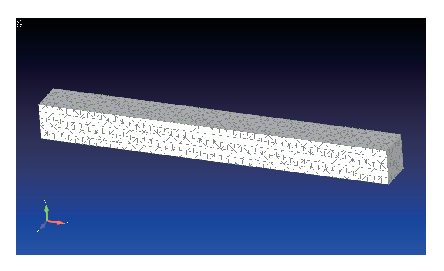
\includegraphics{analysis_eg_init.eps}
	\caption{形状最適化前のモデル} \label{fg:analysis_eg_init}
\end{figure}
今回は概要なので,細かい設定の説明は省きます.
このモデルの右端に鉛直下向きの力を加えたとき,体積制約付きで剛性を最大化する
という形状最適化問題を考えます.
図\ref{fg:analysis_eg_result}は,AzLibを使ってこの最適化問題を解いたときの
最適形状です.
\begin{figure}
	\centering 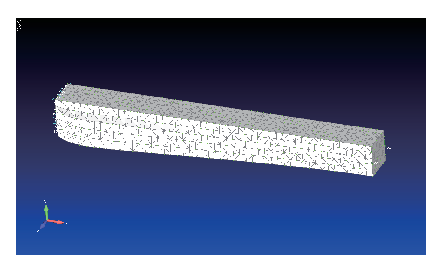
\includegraphics{analysis_eg_result.eps}
	\caption{形状最適化後のモデル} \label{fg:analysis_eg_result}
\end{figure}
このような最適化を行うプログラムを開発する際の土台となるのがAzLibということに
なります.

% 章の役割
畔上研究室の理論では,最適化の実装に有限要素法を用いています.
有限要素法には,行列演算をはじめとする数多くの数値計算が用いられます.
また,あらゆる処理に対してエラーが発生したときの対応もしなければなりません.
さらに,有限要素法は要素の情報の格納に膨大なメモリを必要とするので,使用する
メモリを適切に管理しなければなりません.
最適化の実装にあたって,多くの要件を満たさなければならないのです.
そのため,プログラムを役割ごとにいくつかのディレクトリに分けて,見通しをよく
しています.

まず,\ref{sec:abstract_directory}節ではそれぞれのディレクトリの役割について
説明します. 
次に,\ref{sec:abstract_usage}節ではAzLibの利用法について説明します. 
最後に,\ref{sec:abstract_develop}節ではAzLibの開発方法について説明します.

\section{各ディレクトリの概要} \label{sec:abstract_directory}
ここでは,AzLibを構成するディレクトリの概要を説明します.

AzLibのソースコードの本体はSubversion/azlib/trunk/srcにあります.
実際に見てみると,次の $5$ つのディレクトリがあります.
\begin{itemize}
	\item base
	\item fem
	\item gui
	\item image
	\item mathematics
\end{itemize}

baseディレクトリには,あらゆる処理の土台(base)となるソースコードが含まれて
います.
たとえば,不適切な処理を行わないようにするエラーチェックの仕組みや,使用する
メモリの管理を行う仕組みなどが実装されています.

femディレクトリには,有限要素法の処理に関するソースコードが含まれています.

guiディレクトリには,(執筆中)

imageディレクトリには,(執筆中)

mathematicsディレクトリには,femディレクトリで用いる有限要素法の処理で必要と
なる数値計算に関するソースコードが含まれています.

以上 $5$ つのディレクトリには,図\ref{fg:abstract_hierarchy}のような階層構造が
あることがなんとなくわかると思います.
\begin{figure}
	\centering 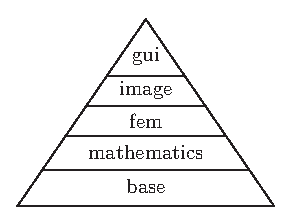
\includegraphics{abstract_hierarchy.eps}
	\caption{AzLibのディレクトリの階層構造} \label{fg:abstract_hierarchy}
\end{figure}
つまり,baseディレクトリのソースコードを土台にしてmathematicsディレクトリの
ソースコードが書かれており,mathematicsディレクトリのソースコードを土台にして
femディレクトリのソースコードが書かれており,・・・ということです.
第\ref{chap:base}章からはそれぞれのディレクトリの中身を説明しますが,
この階層構造で土台となるディレクトリから順に説明していくことにします.


\section{利用方法} \label{sec:abstract_usage}
ここでは,AzLibの使い方を説明します.

\ref{sec:abstract_directory}節で説明したそれぞれのディレクトリの中を見ると
わかりますが,ソースコードはすべてC言語で書かれています.
C言語については,Webで検索すればいくらでも情報が得られます.
そのため,本書ではC言語の基礎についての説明を省きます.

また,コンパイルはすべてmakefileを利用して行います.
makefileについてもWebで情報が得られるので,説明を省きます.
よくわからなければ,わかっている人に聞きましょう.
gccを用いてコンパイルするので,dnfでインストールしておいてください.

\subsection{基本的な使い方}
最適化の手続き本体は,main関数の中で記述することになります.
ここでは例を通して,AzLibを使って最適化を行うプログラムのソースコードを
眺めながら,実際にコンパイルしてみましょう.
今回は,Linuxの端末上でコンパイルすることを前提として説明します.

本章のはじめに簡単な最適化の例を見ましたが,この最適化のソースコードは
Subversion/azlib/trunk/examples/trac\_methodにあります.
まずは端末を開いてこのディレクトリまで移動し,エディタで最適化を行う
プログラムのソースコードを開いてみましょう.
\begin{verbatim}
    $ cd ~/Subversion/azlib/trunk/examples/trac_method
    $ vim trac_method.c
\end{verbatim}
この例ではエディタとしてvimを使っていますが,好きなものを使ってください.

$5$ 行目から $7$ 行目で,AzLibのbaseディレクトリ,mathematicsディレクトリ,
femディレクトリのヘッダファイルを読み込んでいます.
そこからしばらくは,このソースコードで独自に定義しているマクロや構造体,関数の
プロトタイプ宣言が続きます.
そして $69$ 行目から,main関数で最適化の手続きを記述しています.
以降ではプログラムにおける最適化の流れを確認し,実際に実行してみます.

\subsection{最適化の手続き}
main関数の中を簡単に説明します.
最適化の解析は,有限要素法を用いて行います.
はじめに解析するモデルの要素や節点などのデータを読み込み,最適化の
アルゴリズムを実行して,最後に最適化後のモデルのデータを出力します.

要素や節点などのデータは独自の構造体で管理します.
たとえば,$73$ 行目の\texttt{NODE\_ARRAY}型変数\texttt{node}で節点のデータを,
$74$ 行目の\texttt{ELEMENT\_ARRAY}型変数\texttt{element}で要素のデータを
管理します.
この他にも,有限要素法に関係のあるデータのほとんどが構造体で管理されます.
詳しくは,\ref{chap:fem}章で説明します. % そのうち節番号に変更する

$94$ 行目では,ログの出力の量を調節する「ログ出力レベル」の設定をしています.
続く $97$,$98$,$99$ 行目では,そのログの出力先を設定しています.
ログ出力の詳細については,\ref{sec:log-output-utl}節で説明します.

ここで,ログ出力レベルの設定に使っている関数の呼び出し方を見てみましょう.
AzLibには,RC型と呼ばれる独自の変数の型があります.
main関数でRC型の関数を用いるときは,このように「\texttt{RC\_TRY\_MAIN}」
マクロを利用します.
RC型の詳細については,\ref{subsec:RC-type}節で説明します.

$102$ 行目では,解析で使用するメモリの上限値を設定しています.
十分な量のメモリを確保して,以降の解析を行います.

$105$ 行目から $132$ 行目までは,解析に関するパラメータやモデルのデータを変数に
格納しています.
このあたりは,どのような最適化プログラムでも同様の記述になるはずです.

$135$ 行目から $144$ 行目で,解析結果を書き出すファイルを用意しています.
直後の最適化の処理には,場合によっては膨大な時間がかかります.
最適化の処理を実行した後で「結果をファイルに書き出せません」ということに
ならないよう,最適化の処理の前でこれらのファイルを用意します.

$146$ 行目から $149$ 行目で,最適化を実行します.
main関数の下にある\texttt{optimization()}という関数に,最適化の
アルゴリズムを記述しています.

$152$ 行目から $165$ 行目で,最適化したモデルを出力しています.

$169$ 行目で,$102$ 行目で動的確保したメモリを解放しています.

以上のような流れで,最適化を実行しています.
今回は線形弾性体の形状最適化を行うプログラムの例でしたが,どのような
最適化でもmain関数の中は同様になると考えられるので,プログラムを書くときには
参考になると思います.

\subsection{最適化プログラムのコンパイル}
最後に,このソースコードのコンパイルをしてみましょう.
このディレクトリにはmakefileがすでにあり,\verb|make|を実行するだけでコンパイルが
できるようになっています.
実際にコンパイルしてみましょう.
\begin{verbatim}
    $ make
\end{verbatim}

\verb|make|を実行するだけだとコンパイルの手順がややわかりづらいので,少しだけ
説明しておきます.
\verb|make|を実行すると,まず本体のソースコードのオブジェクトファイルを
生成します.
次に,AzLibの各ディレクトリごとのライブラリファイルを生成します.
このとき,各ディレクトリごとに用意されているmakefileを使います.
必要なライブラリファイルを生成したら,それらをリンクして実行モジュールを生成
します.
trac\_method内のmakefileは,この一連の手順を行うように記述されています.

どのようなソースコードを書いても,makefileの基本的な書き方はほとんど
変わりません.
自分でソースコードを書いた場合も,このmakefileをコピーしたものを少し書き換える
だけで済むはずです.

この例の最適化プログラムは,通常のC言語の実行ファイルと同じ方法で実行します.
ただしmain関数に渡す引数がいくつかあるので,実行するためのスクリプトがあります.
実際はこのスクリプトを実行すれば,ソースコードのコンパイルから実行ファイルの実行
までをすべて行ってくれます.
run.shというファイルが実行のスクリプトなので,実行してみましょう.
\begin{verbatim}
    $ ./run.sh
\end{verbatim}

形状更新などの履歴を適度に出力しながら最適化を行う様子がわかると思います.
このようなログを出力することも,プログラムに求められることのひとつです.
ログの出力の仕組みは,baseディレクトリで実装されています.


\section{開発方法} \label{sec:abstract_develop}
ここでは,AzLibの開発方法を説明します.

AzLibはSubversionによってソースコードを一元的に管理しています.
(執筆中)

